% 图 13.2 —— 由 `checks/emit_hand.py` 自动拼出（probe 精测 + prims2 图元分解）
%%
% ⚠ 这是**稿子不是成品**：跑 `checks/checkhand.py 13.2` 看指标 + 看叠合图。
%%
%% ⚠ 待核：
%   · 本图 probe 报出阴影族 1 个 —— **本脚本不生成阴影**（要照原书手写）；prims2 的 strokes 里可能含阴影线，核对时留意别画重
%   · 可疑字形 1 项（空心圈 ⊙ 常被认成字母 o）—— 见文件末
%%
\documentclass[12pt]{standalone}
\usepackage{fontspec}
\setsansfont{Arial}
\newfontfamily\mfallback{DejaVu Sans}
\usepackage{tikz}
\begin{document}
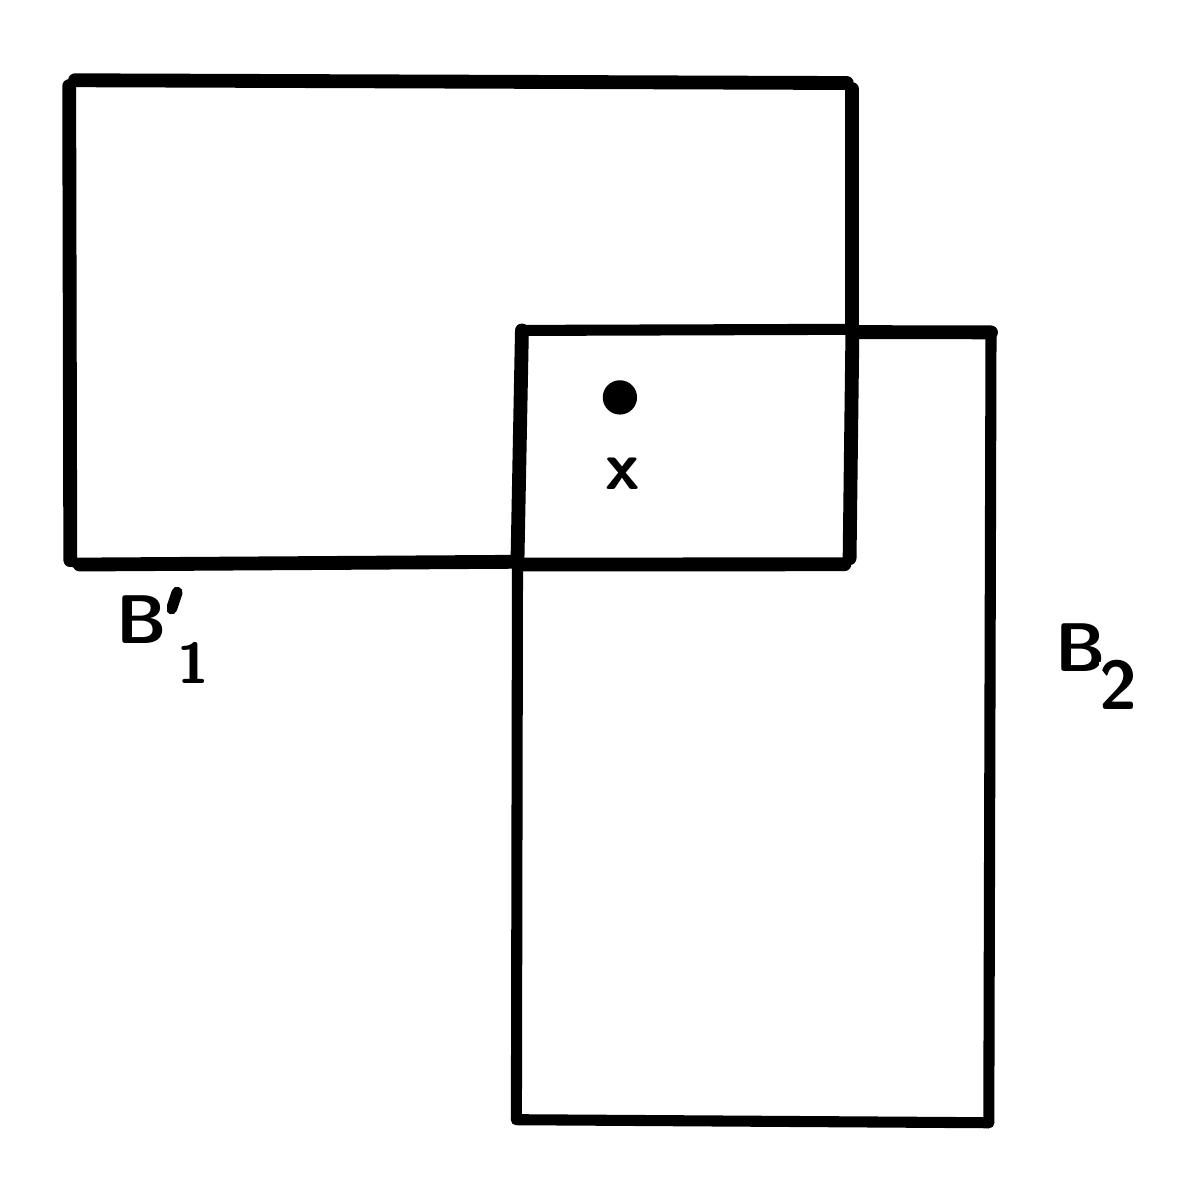
\begin{tikzpicture}[x=1pt, y=-1pt, line width=5.0pt, line cap=round, line join=round]

  %% ════ 填充区（prims2 的 fills）════

  %% ════ 直线段（prims2 的 strokes）════
  \draw[line width=5.0pt] (176.0,193.0) -- (18.8,194.0);
  \draw[line width=3.9pt] (18.8,194.0) -- (15.4,192.4);
  \draw[line width=5.0pt] (15.4,192.4) -- (15.0,21.1);
  \draw[line width=3.0pt] (15.0,21.1) -- (17.1,19.0);
  \draw[line width=5.0pt] (17.1,19.0) -- (296.0,20.0);
  \draw[line width=2.9pt] (296.0,20.0) -- (298.0,22.2);
  \draw[line width=5.0pt] (298.0,22.2) -- (298.0,108.0);
  \draw[line width=4.0pt] (52.0,210.0) -- (54.0,204.0);
  \draw[line width=5.0pt] (177.0,192.0) -- (178.6,109.4);
  \draw[line width=4.0pt] (178.6,109.4) -- (297.0,109.0);
  \draw[line width=4.0pt] (177.0,195.0) -- (176.6,394.6);
  \draw[line width=4.0pt] (176.6,394.6) -- (347.3,395.7);
  \draw[line width=4.0pt] (347.3,395.7) -- (348.1,110.1);
  \draw[line width=5.0pt] (348.1,110.1) -- (299.0,110.0);
  \draw[line width=5.0pt] (298.0,111.0) -- (297.0,191.7);
  \draw[line width=2.9pt] (297.0,191.7) -- (295.1,193.9);
  \draw[line width=5.0pt] (295.1,193.9) -- (178.0,194.0);

  %% ════ 实心点 ════
  \fill (214.0,133.6) circle (6.2);

  %% ════ 标签（probe 直接给的 \node 行）════
  %% ⚠ 全部补了 fill=white：文字在最上层，否则与曲线交叉干扰
     \node[anchor=center,inner sep=0pt,fill=white,font=\fontsize{30.1}{37.6}\selectfont] at (215.0,161.0) {\textsf{\textbf{\textit{x}}}};   % box(206,150,16,18)
     \node[anchor=center,inner sep=0pt,fill=white,font=\fontsize{30.2}{37.8}\selectfont] at (41.3,214.0) {\textsf{\textbf{\textit{B}}}};   % box(30,202,19,23)
     \node[anchor=center,inner sep=0pt,fill=white,font=\fontsize{36.1}{45.1}\selectfont] at (380.6,224.1) {\textsf{\textbf{\textit{B}}}};   % box(365,212,27,23)
     \node[anchor=center,inner sep=0pt,fill=white,font=\fontsize{21.5}{26.9}\selectfont] at (60.0,229.9) {\textsf{\textbf{1}}};   % box(54,222,7,15)
     \node[anchor=center,inner sep=0pt,fill=white,font=\fontsize{23.6}{29.6}\selectfont] at (394.1,237.9) {\textsf{\textbf{2}}};   % box(388,229,11,17)

  % 钉死画布：否则超出的图元/控制点会把页面撑大，1:1 回比就失准
  \pgfresetboundingbox
  \path[use as bounding box] (0,0) rectangle (408,408);
\end{tikzpicture}
\end{document}

% ⚠ 待核清单（probe 拿不准，人眼过一遍）：
%   · 未识别/跳过：⑤ 跳过/未识别的字形
